\documentclass[conference]{IEEEtran}
\IEEEoverridecommandlockouts

\usepackage[utf8]{inputenc}
\usepackage{amsmath}
\usepackage{amssymb}
\usepackage{graphicx}
\usepackage{cite}
\usepackage{url}
\usepackage{booktabs}
\usepackage{multirow}
\usepackage{color}
\usepackage{hyperref}

% For better figure placement
\usepackage{float}

\title{Remaining Useful Life Estimation of Turbofan Engines Using Machine Learning}

\author{\IEEEauthorblockN{Felix Ikokwu\IEEEauthorrefmark{} and Hunter Antal\IEEEauthorrefmark{}}
\IEEEauthorblockA{\IEEEauthorrefmark{}Faculty of Engineering, Lakehead University, Thunder Bay, ON P7B 5E1, Canada\\
Email: feikokwu@lakeheadu.ca, hbantal@lakeheadu.ca}}

\begin{document}

\maketitle

\begin{abstract}
Predictive maintenance is widely used to reduce unexpected equipment failure and improve system reliability. One important task in predictive maintenance is Remaining Useful Life (RUL) prediction, which estimates how many operational cycles remain before a system fails. This project focuses on developing and comparing machine learning and neural network models for RUL prediction using time-series sensor data. The NASA Turbofan Engine Degradation dataset is used as a benchmark dataset. Several models with increasing complexity are implemented and evaluated based on prediction accuracy and computational cost. The goal of this project is to understand the trade-offs between model performance and complexity while demonstrating an end-to-end computational intelligence workflow.
\end{abstract}

\begin{IEEEkeywords}
Remaining Useful Life, predictive maintenance, machine learning, neural networks, time-series data
\end{IEEEkeywords}

\section{Introduction}

\subsection{Background}
Industrial systems naturally degrade over time due to continuous operation and environmental conditions. If degradation is not monitored, it can lead to unexpected failures, increased maintenance costs, and safety concerns. Predictive maintenance aims to address these issues by using historical data to identify early signs of failure and support timely maintenance decisions.

Remaining Useful Life (RUL) prediction is a key predictive maintenance task that estimates how long a system can continue operating before failure \cite{ref1}. Recent advances in machine learning and neural networks have enabled the modeling of complex degradation patterns using multivariate sensor data, and prior work has shown that these approaches are well suited for RUL estimation problems \cite{ref3}.

Neural networks, in particular, are effective at capturing nonlinear relationships and temporal trends in time-series data.

\subsection{Problem Definition}
The objective of this project is to predict the Remaining Useful Life of turbofan engines using historical sensor measurements collected during operation. Given a sequence of sensor readings and operational settings, the prediction problem will be explored as a supervised regression problem. The model output will be a continuous value representing the number of operational cycles remaining before engine failure.

In this project, several machine learning and neural network models will be applied to the RUL prediction problem and compared to evaluate their predictive performance and computational efficiency. This comparison will allow for an assessment of how increasing model complexity influences accuracy and resource requirements within a predictive maintenance context.

\section{Dataset Description}

The NASA Turbofan Engine Degradation dataset, also known as the C-MAPSS dataset, will be used in this project. The NASA Prognostics Center of Excellence provides this dataset and is commonly used for benchmarking RUL prediction methods \cite{ref2}\cite{ref5}.

The dataset consists of multiple run-to-failure simulations of turbofan engines. For each engine, sensor measurements are recorded at every operational cycle. The dataset includes:

\begin{itemize}
    \item Engine unit identifiers
    \item Cycle numbers
    \item Three operational settings
    \item Twenty-one continuous sensor measurements
\end{itemize}

The training dataset contains complete degradation histories for approximately 100 engines, while the test dataset includes partial degradation data for different engines. This structure makes the dataset well-suited for evaluating machine learning and neural network approaches to RUL prediction.

\section{Input Features and Target Variable}

\subsection{Input Features}
The input features include numerical sensor readings and operational settings recorded at each cycle. During preprocessing, additional features such as windowed sensor sequences may be created to better represent temporal behaviour.

\subsection{Target Variable}
The target variable is Remaining Useful Life, defined as the number of cycles remaining until engine failure. RUL is treated as a continuous numerical value, and the problem is approached as a regression task.

\section{Proposed Models}

To compare different modeling techniques, three models were developed:

\begin{itemize}
    \item \textbf{Baseline Model:} A classical machine learning model, Random Forest Regression, was used to establish baseline performance.

    \item \textbf{Neural Network Model:} A Multilayer Perceptron (MLP) was implemented to capture nonlinear relationships between the input features and RUL.

    \item \textbf{Advanced Neural Network Model:} A Long Short-Term Memory (LSTM) network was used to model temporal dependencies in the sensor time-series data \cite{ref4}.
\end{itemize}

\section{Evaluation Metrics}

Model performance was evaluated using standard regression metrics, including:

\begin{itemize}
    \item Mean Absolute Error (MAE)
    \item Root Mean Squared Error (RMSE)
    \item R-squared (R$^2$)
\end{itemize}

In addition, model efficiency was assessed using:

\begin{itemize}
    \item Number of trainable parameters
    \item Inference time
    \item Estimated floating-point operations (FLOPs)
\end{itemize}

\section{Exploratory Data Analysis}

\subsection{Data Preprocessing and Preparation}

The C-MAPSS dataset contains a large selection of simulated engine degradation data, split into various subsets. For this study, the FD001 subset was selected for preprocessing and model training. This section focuses on the methodologies employed to prepare the dataset for further analysis and model training.

\subsubsection{Dataset Visualization}
Before performing any significant transformations on the dataset, the raw data was first visualized using a histogram. This allowed for an initial exploration of the dataset beyond the provided text file. Upon examining the data visualization, it is evident that certain feature values are constant.

\begin{figure*}[h]
    \centering
    \includegraphics[width=\textwidth]{figures/fig1.png}
    \caption{Raw Data Variance Visualization}
    \label{fig:raw_variance}
\end{figure*}

\begin{figure*}[h]
    \centering
    \includegraphics[width=\textwidth]{figures/fig2.png}
    \caption{Raw Sensor Data In Small Multiples}
    \label{fig:raw_sensors}
\end{figure*}

\subsubsection{Feature Selection}
Following the raw data visualization, feature selection was performed using Equations \eqref{eq:variance}--\eqref{eq:correlation} (for variance, covariance, and correlation metrics, respectively) to validate the conclusions drawn from the visualizations. This step also helped in identifying and retaining the most informative features for predicting RUL. Features with low variance, low covariance, and low correlation with the target variable (RUL) were removed to improve model performance. The following features were excluded:

\begin{itemize}
    \item Operational Settings: operational\_setting\_2, operational\_setting\_3
    \item Sensors: sensor\_1, sensor\_5, sensor\_6, sensor\_10, sensor\_16, sensor\_18, sensor\_19
\end{itemize}

This approach ensured that only the most relevant features were kept, preventing the inclusion of irrelevant or redundant data that would otherwise decrease model performance.

The variance for each feature was calculated using the formula:

\begin{equation}
\text{Variance} = \frac{1}{N - 1} \sum_{i=1}^{N} \left( x_i - \mu \right)^2
\label{eq:variance}
\end{equation}

where $x_i$ represents individual feature values, $N$ is the number of data points, and $\mu$ is the mean of the feature. Features with a variance below a threshold of 0.01 were removed.

Covariance was computed between each feature and the RUL using the equation:

\begin{equation}
\text{Cov}(X,Y) = \frac{1}{N} \sum_{i=1}^{N} \left( x_i - \overline{X} \right) \left( y_i - \overline{Y} \right)
\label{eq:covariance}
\end{equation}

where $X$ and $Y$ are the two variables (feature and RUL), and $\overline{X}$ and $\overline{Y}$ are the means of $X$ and $Y$. Features with a covariance below 0.1 were discarded.

The correlation between each feature and RUL was calculated using the formula:

\begin{equation}
\text{Correlation}(X,Y) = \frac{\text{Cov}(X,Y)}{\sigma_X \sigma_Y}
\label{eq:correlation}
\end{equation}

where $\sigma_X$ and $\sigma_Y$ are the standard deviations of $X$ and $Y$. Features with a correlation coefficient of less than 0.3 were also removed.

\subsubsection{LSTM Windowing}
After feature selection, the cleaned dataset was transformed into sequences of cycles using a sliding window approach \cite{ref6}\cite{ref7} to prepare it for the LSTM model. In this approach, each window contains 30 consecutive cycles of data, with the target variable (RUL) assigned as the last RUL value of the final cycle in the window.

Windowing was selected because LSTMs are designed to learn from sequences of data, which capture temporal dependencies within the dataset. A window size of 30 cycles was chosen, falling between the 10--15\% range of the average engine cycle mean. This size allows the model to capture sufficient context for pattern recognition over time.

\subsubsection{Normalization}
Normalization was applied to ensure that all features were on the same scale. Given that the raw data contained features with varying numeric ranges, standardization was performed using Eq. \eqref{eq:normalization} to scale the data such that each feature had a mean of 0 and a standard deviation of 1. This step ensured that no feature dominated the model training due to its scale, enabling fair and efficient learning.

\begin{equation}
X_{\text{norm}} = \frac{X - \mu}{\sigma}
\label{eq:normalization}
\end{equation}

where $X$ is the original feature value, $\mu$ is the mean of the feature, and $\sigma$ is the standard deviation of the feature. This method was chosen because neural networks (such as LSTMs) perform better and converge faster when the input features are scaled to the same range.

\subsection{Results of Preprocessing}

The data preprocessing resulted in the reduction of 24 raw features to 15 normalized features. A comparison between the normalized features and the raw data is shown in Fig. \ref{fig:normalized_features}. The remaining 15 features have been normalized to have a mean of 0 and a standard deviation of 1, which is ideal for model training. All 15 features meet the required thresholds for variance, covariance, and correlation. These features are now ready to contribute to the model's understanding.

\begin{figure*}[h]
    \centering
    \includegraphics[width=\textwidth]{figures/fig3b.png}
    \caption{Raw Data - Un-Normalized (Original) Features}
    \label{fig:unnormalized_features}
\end{figure*}

\begin{figure*}[h]
    \centering
    \includegraphics[width=\textwidth]{figures/fig3a.png}
    \caption{Data After Normalization - Normalized (Green) Selected Features}
    \label{fig:normalized_features}
\end{figure*}

\section{Model Evaluation and Comparison}

This section presents the evaluation of the selected models: a classical baseline model, a multilayer perceptron (MLP), and a Long Short-Term Memory (LSTM) network. Each model is assessed using regression performance metrics, residual analysis, and prediction behaviour. A final comparison is then performed to determine the model selected for continuation of the project.

\subsection{Baseline: Random Forest Regression}

Random Forest regression was selected as the primary classical baseline model due to its ability to model nonlinear relationships without requiring explicit feature engineering. As an ensemble of decision trees trained on bootstrapped subsets of the data, Random Forest reduces variance through averaging while maintaining flexibility in capturing nonlinear dependencies between features and RUL.

Unlike Linear Regression, which assumes a linear relationship of the form shown in Eq. \eqref{eq:linear_reg}, Random Forest constructs piecewise constant approximations of the regression function through recursive partitioning of the feature space. This makes it suitable for high-dimensional tabular inputs derived from flattened windowed sequences.

\begin{equation}
\hat{y} = \beta_0 + \beta_1 x_1 + \cdots + \beta_p x_p
\label{eq:linear_reg}
\end{equation}

Since the model does not explicitly model temporal order, each input window of dimension $30 \times 15$ was flattened to a 450-dimensional feature vector. This transformation was necessary because tree-based models operate on fixed-length tabular inputs rather than structured time series tensors. Introducing flattening preserves all numerical information within windows but removes explicit temporal structure.

\subsubsection{Quantitative Performance}
Validation performance was conducted using the proposed metrics of MAE, RMSE, and R$^2$, which produced the following results:

\begin{itemize}
    \item MAE = 14.014
    \item RMSE $\approx$ 19.579
    \item R$^2$ $\approx$ 0.778
\end{itemize}

The relatively high R$^2$ indicates that the model explains a substantial portion of the variance in RUL. However, the RMSE suggests notable prediction deviation for certain regions.

\subsubsection{Predicted vs Actual Analysis}
The predicted versus actual RUL scatter plots for the validation and test sets are shown in Fig. \ref{fig:rf_scatter}. The red dashed diagonal represents perfect prediction, where:

\begin{equation}
\text{predicted RUL} = \text{actual RUL}
\label{eq:perfect_pred}
\end{equation}

Points lying directly on this line indicate exact agreement between predicted and actual RUL values.

Points above the diagonal represent overprediction, where:

\begin{equation}
\hat{y} > y
\label{eq:overpred}
\end{equation}

In this case, the model predicts a higher RUL than the true value, implying that the engine is estimated to be healthier than it actually is.

Conversely, points below the diagonal represent underprediction, where:

\begin{equation}
\hat{y} < y
\label{eq:underpred}
\end{equation}

In this scenario, the model predicts an RUL lower than the true value, implying that the engine is estimated to be closer to failure than it truly is.

\begin{figure}[H]
    \centering
    \includegraphics[width=0.95\linewidth]{figures/fig4.png}
    \caption{Predicted vs. Actual RUL - Random Forest}
    \label{fig:rf_scatter}
\end{figure}

In the early degradation region (actual RUL = 115--130 cycles), a noticeable compression of predictions is observed. Many points fall below the diagonal, indicating systematic underprediction at high RUL values. This suggests that the model tends to estimate engines as being closer to degradation than they truly are during early-life stages. The vertical clustering near the upper RUL bound further indicates limited sensitivity to subtle variations in healthy operating conditions.

In the late degradation region (actual RUL = 0--30 cycles), predictions align more closely with the diagonal; however, variance increases as RUL approaches zero. Both overprediction and underprediction are present, though the spread remains comparatively smaller than in the high-RUL region. From a maintenance perspective, overprediction in this region is particularly critical, as it implies estimating more remaining life than is actually available.

Across the mid-range RUL values ($\approx$ 30--100 cycles), dispersion around the diagonal increases, indicating reduced prediction consistency as degradation progresses. This widening spread reflects the model's difficulty in capturing the transitional behaviour between early and late degradation stages.

Overall, while the model captures the global nonlinear relationship between sensor inputs and RUL, the observed compression at high RUL values and increasing variance in the mid-range indicate limitations in representing degradation progression. Since the Random Forest model operates on flattened inputs without explicit temporal awareness, sequential degradation patterns must be inferred indirectly rather than modeled.

\subsubsection{Residual Analysis}
The residual distributions for the validation and test sets are shown in Fig. \ref{fig:rf_residuals}. Residuals are defined as:

\begin{equation}
e = y - \hat{y}
\label{eq:residuals}
\end{equation}

where $y$ represents the true RUL and $\hat{y}$ the predicted RUL. A residual of zero indicates perfect prediction. Positive residuals correspond to underprediction ($\hat{y} < y$), while negative residuals correspond to overprediction ($\hat{y} > y$).

\begin{figure}[H]
    \centering
    \includegraphics[width=0.95\linewidth]{figures/fig5.png}
    \caption{RF Residual Distribution: Validation vs. Test Results}
    \label{fig:rf_residuals}
\end{figure}

The validation set exhibits a mean residual of approximately $-1.4$ cycles, while the test set shows a mean residual of approximately $+2.3$ cycles. The near-zero mean in the validation set indicates limited systematic bias during training. The slight positive shift in the test set suggests mild underprediction on unseen data. Although this shift is small relative to the overall RUL range, it indicates minor generalization drift.

The residual distributions are not perfectly symmetric and display heavier tails, particularly in the negative region. This implies that larger overpredictions occur more frequently than large underpredictions within certain RUL intervals. Additionally, the spread of residuals increases as RUL increases, indicating heteroscedastic behaviour. This observation is consistent with the predicted versus actual plots, where higher RUL values exhibit greater dispersion.

Operationally, residual direction has practical implications: large negative residuals in low-RUL regions represent overestimation of remaining life and thus pose a greater maintenance risk. Conversely, large positive residuals correspond to conservative predictions that may lead to premature maintenance scheduling. The observed distribution suggests that the Random Forest model maintains moderate bias control but exhibits non-uniform error variance across degraded stages.

\subsubsection{Hyperparameter Sensitivity}
The hyperparameter sensitivity analysis for the Random Forest model is shown in Fig. \ref{fig:rf_heatmap}, where validation RMSE is evaluated across varying values of \textit{max\_depth} and \textit{n\_estimators}. These two parameters control the expressive capacity and ensemble stability of the model.

\begin{figure}[H]
    \centering
    \includegraphics[width=0.95\linewidth]{figures/fig6.png}
    \caption{Heat Map of RF Hyperparameters}
    \label{fig:rf_heatmap}
\end{figure}

The parameter \textit{max\_depth} governs the maximum depth of individual decision trees. Increasing tree depth allows the model to capture more complex nonlinear relationships but may increase variance. The parameter \textit{n\_estimators} controls the number of trees in the ensemble, with larger values generally reducing variance through averaging.

The heatmap indicates minimal variation in RMSE across the tested hyperparameter combinations. Performance stabilizes around RMSE $\approx 19.6$, with only marginal improvements observed for deeper trees and larger ensembles. This suggests that the model has reached a representational plateau under the current input structure.

The limited sensitivity to hyperparameter adjustments implies that the dominant error source is not insufficient tree depth or ensemble size, but rather structural constraints of the model. Thus, increasing model complexity within the Random Forest framework does not substantially improve predictive accuracy for this dataset. This behaviour further illustrates that while Random Forest effectively captures nonlinear feature interactions, additional modeling complexity is insufficient to significantly reduce error without incorporating temporal data.

\subsection{Multilayer Perceptron (MLP)}

The MLP was implemented to evaluate whether learned nonlinear feature transformations improve RUL prediction compared to the classical baseline. Unlike Random Forest, which partitions feature space using tree structures, the MLP learns a parametric mapping through stacked fully connected layers with nonlinear activation functions.

The selected configuration consisted of three hidden layers with dimensions $[64, 128, 64]$, a learning rate of $0.001$, and a dropout rate of $0.3$. The total number of trainable parameters was $18,177$. Dropout regularization was applied to mitigate overfitting by randomly deactivating neurons during training.

\subsubsection{Quantitative Performance}
The best-performing MLP configuration achieved the following results:

\textbf{Validation set:}
\begin{itemize}
    \item MAE = 13.504
    \item RMSE = 18.946
    \item R$^2$ = 0.7918
\end{itemize}

\textbf{Test set:}
\begin{itemize}
    \item MAE = 12.067
    \item RMSE = 16.892
    \item R$^2$ = 0.6249
\end{itemize}

Compared to the Random Forest baseline, MLP demonstrates a modest improvement in validation RMSE and MAE. The validation R$^2$ also increased slightly, indicating improved variance explanation during training. However, the decrease in test R$^2$ performance suggests reduced generalization stability compared to validation performance. While absolute test errors improved in terms of RMSE and MAE, the reduced R$^2$ indicates sensitivity to unseen degradation patterns. Overall, MLP provides incremental accuracy gain but does not fully resolve generalization limitations.

\subsubsection{Predicted vs Actual Analysis}
The predicted versus actual RUL scatter plots for the validation and test sets are shown in Fig. \ref{fig:mlp_scatter}. Starting at the early degradation region (actual RUL $\approx 115$--$130$), predictions remain compressed near the upper bound. However, compared to the Random Forest model, the clustering around the diagonal is tighter, indicating improved consistency at high RUL values.

\begin{figure}[H]
    \centering
    \includegraphics[width=0.95\linewidth]{figures/fig7.png}
    \caption{Predicted vs. Actual RUL - Multilayer Perceptron}
    \label{fig:mlp_scatter}
\end{figure}

In the mid-range region ($\approx 30$--$100$ cycles), dispersion is reduced relative to the baseline, suggesting that nonlinear feature transformations improve representation of transitional degradation behaviour. Finally, in the late degradation region ($\approx 0$--$30$ cycles), predictions align closely with the diagonal, though some overprediction remains visible. Similar to the baseline model, overprediction in this region corresponds to estimating greater remaining life than is actually available.

Overall, the MLP demonstrates improved alignment with the diagonal across most RUL ranges, but upper-bound compression persists, indicating limitations in modeling subtle early-life degradation signals.

\subsubsection{Residual Analysis}
The residual distributions for the validation and test sets are shown in Fig. \ref{fig:mlp_residuals}.

\begin{figure}[H]
    \centering
    \includegraphics[width=0.95\linewidth]{figures/fig8.png}
    \caption{MLP Residual Distribution: Validation vs. Test Results}
    \label{fig:mlp_residuals}
\end{figure}

The validation residual mean is approximately $-0.2$ cycles, indicating near-zero bias during training. The test residual mean is approximately $3.8$ cycles, indicating moderate underprediction on unseen data. Compared to the Random Forest model, the validation residual distribution is more tightly centred around zero, suggesting improved bias control. However, the test distribution exhibits increased asymmetry and a heavier positive tail, indicating a greater frequency of underprediction in certain regions. Residual spread remains larger at higher RUL values, confirming that early degradation stages continue to exhibit greater uncertainty. Thus, while the MLP reduces validation bias and slightly improves predictive consistency, residual variance remains non-uniform across degradation stages.

\subsubsection{Hyperparameter Sensitivity}
The hyperparameter sensitivity of MLP is illustrated in Fig. \ref{fig:mlp_heatmap}, which presents validation RMSE across varying hidden layer architectures, learning rates, and dropout configurations. The corresponding training dynamics are shown in Fig. \ref{fig:mlp_training}.

\begin{figure}[H]
    \centering
    \includegraphics[width=0.95\linewidth]{figures/fig9.png}
    \caption{Heat Map of MLP Hyperparameters}
    \label{fig:mlp_heatmap}
\end{figure}

The heatmap reveals that the architecture $[64, 128, 64]$ consistently achieves the lowest validation RMSE, with a minimum value of approximately $18.934$ when dropout $= 0.2$ and learning rate $= 0.0005$. This symmetric bottleneck structure balances representational capacity and overfitting effectively. Increasing network width to $[256, 128, 64]$ does not improve performance and slightly increases RMSE, suggesting that additional parameters introduce variance without improving generalization.

Dropout sensitivity is also evident. Increasing the dropout rate from $0.2$ to $0.3$ generally results in higher validation RMSE across architectures. While dropout mitigates overfitting by randomly deactivating neurons, excessive regularization of this type constrains the network's ability to learn meaningful nonlinear feature interactions from the flattened input representation.

Minor variations in the learning rate, specifically between $0.0005$ and $0.001$, resulted in only marginal differences in the validation RMSE. This suggests that the optimization process is sufficiently stable for convergence within this range, indicating that the architectural design is a more significant determinant of the final performance than the precise learning rate setting.

\begin{figure}[H]
    \centering
    \includegraphics[width=0.95\linewidth]{figures/fig10.png}
    \caption{Loss vs. Epoch - MLP Training}
    \label{fig:mlp_training}
\end{figure}

The training curve further supports this understanding, as training loss decreases rapidly during the initial epochs and stabilizes after approximately $15$ epochs, while validation RMSE follows a similar trajectory without significant divergence. The absence of widening gaps between training and validation curves suggests that the selected configuration achieves stable convergence without any severe overfitting.

Overall, the hyperparameter search indicates that MLP's performance is moderately sensitive to architectural configuration and regularization strength, but relatively robust to small learning rate variations. However, the performance gains across configurations remain confined within a narrow RMSE range (approximately $18.9$--$19.2$ cycles), suggesting that improvements from increased fully connected capacity are incremental rather than structural.

\subsection{Long Short-Term Memory (LSTM)}

The LSTM model was implemented to explicitly capture temporal dependencies within the degradation sequences. Unlike the Random Forest and MLP models, which treat each cycle independently as a flat feature vector with no temporal context, the LSTM processes input sequences of shape (Timesteps, Features), preserving temporal ordering across cycles.

The selected configuration consisted of:
\begin{itemize}
    \item Hidden size: 128
    \item Number of layers: 1
    \item Dropout rate: 0.2
    \item Total parameters: 82,561
\end{itemize}

The substantially larger parameter count reflects the recurrent gating mechanisms inherent to LSTM architecture, thus enabling memory retention and sequential state updates.

\subsubsection{Quantitative Performance}
The best-performing LSTM configuration achieved:

\textbf{Validation set:}
\begin{itemize}
    \item MAE = 9.206
    \item RMSE = 13.348
    \item R$^2$ = 0.8982
\end{itemize}

\textbf{Test set:}
\begin{itemize}
    \item MAE = 10.339
    \item RMSE = 14.759
    \item R$^2$ = 0.7535
\end{itemize}

These results represent a substantial improvement over both the Random Forest and MLP models. Validation RMSE decreases by more than $5$ cycles relative to the MLP, and the validation R$^2$ increases significantly, indicating that the LSTM explains a much larger proportion of variance in RUL. On the test set, performance degradation is modest compared to validation, and the test R$^2$ remains substantially higher than previous models. This indicates improved generalization capacity when modeling degradation progression. The magnitude of improvement suggests that temporal data is a dominant factor in accurate RUL estimation.

\subsubsection{Predicted vs Actual Analysis}
The predicted versus actual RUL plots for validation and test sets are shown in Fig. \ref{fig:lstm_scatter}. Compared to previous models, several structural differences are evident: the dispersion around the diagonal is significantly reduced across the full RUL range; compression in the high-RUL region (early degradation stage) is noticeably mitigated; and mid-range predictions show improved continuity along the diagonal.

\begin{figure}[H]
    \centering
    \includegraphics[width=0.95\linewidth]{figures/fig11.png}
    \caption{Predicted vs. Actual RUL - Long Short-Term Memory}
    \label{fig:lstm_scatter}
\end{figure}

Looking at the early degradation region ($\approx 115$--$130$ cycles), LSTM demonstrates improved sensitivity to subtle sensor variations, reducing routine underprediction observed in prior models. Predictions in the late degradation region ($\approx 0$--$30$ cycles) are still closely aligned with the diagonal. Furthermore, compared to both RF and MLP, there are fewer instances of extreme overprediction in this range. The improved alignment across all degradation stages indicates that sequential memory allows the model to better track progressive degradation rather than infer it from static feature magnitudes.

\subsubsection{Residual Analysis}
The residual distributions for the validation and test sets are shown in Fig. \ref{fig:lstm_residuals}.

\begin{figure}[H]
    \centering
    \includegraphics[width=0.95\linewidth]{figures/fig12.png}
    \caption{LSTM Residual Distribution: Validation vs. Test Results}
    \label{fig:lstm_residuals}
\end{figure}

The validation residual mean is approximately $0.7$ cycles, while the test residual mean is approximately $2.4$ cycles. Both values remain small relative to the full RUL range, indicating minimal systematic bias. More importantly, the residual distributions are noticeably narrower than those of RF and MLP, reflecting reduced prediction variance. The tails are less pronounced, indicating fewer extreme overprediction or underprediction events. Residual spread remains present, but its magnitude is substantially reduced compared to previous models. This reduction in variance confirms that the LSTM more effectively stabilizes prediction error across degradation stages.

\subsubsection{Hyperparameter Sensitivity}
The LSTM hyperparameter sensitivity is illustrated in Fig. \ref{fig:lstm_heatmap}, where validation RMSE is evaluated across varying hidden sizes, dropout rates, and layer depths.

\begin{figure}[H]
    \centering
    \includegraphics[width=0.95\linewidth]{figures/fig13.png}
    \caption{Heat Map of LSTM Hyperparameters}
    \label{fig:lstm_heatmap}
\end{figure}

For a single-layer LSTM, increasing the hidden size from $64$ to $128$ consistently improves performance. The configuration with hidden size $128$ and dropout rate $0.3$ achieves the lowest validation RMSE ($\approx 13.124$). This indicates that additional hidden-state capacity enhances the model's ability to encode temporal degradation patterns.

When the number of layers is increased from one to two, performance does not improve and, in most cases, degrades slightly. Although deeper recurrent stacks theoretically allow hierarchical temporal abstraction, the results suggest that additional depth introduces optimization difficulty or unnecessary variance for this dataset size.

Dropout sensitivity demonstrates a clear pattern: a dropout rate of $0.3$ is generally superior to $0.2$, especially when using larger hidden sizes. In this context, stronger regularization does not limit the network's representation power. Instead, it stabilizes the recurrent state transitions, which effectively mitigates overfitting.

\begin{figure}[H]
    \centering
    \includegraphics[width=0.95\linewidth]{figures/fig14.png}
    \caption{Loss vs. Epoch - LSTM Training}
    \label{fig:lstm_training}
\end{figure}

The LSTM training curve demonstrates rapid loss reduction during early epochs followed by stable convergence. Validation RMSE tracks training loss closely, indicating effective regularization and minimal divergence between training and validation behaviour. A brief fluctuation near epoch $15$ does not lead to sustained instability.

Overall, the hyperparameter search indicates that LSTM performance is primarily influenced by hidden-state dimensionality rather than network depth. Increasing hidden size improves temporal representation capacity, while additional stacked layers provide limited benefit under the current dataset. Importantly, the performance gains observed across configurations are more substantial than those seen in the MLP search, reinforcing the importance of temporal modeling rather than simply increasing fully connected capacity.

\subsection{Model Performance Comparison}

The comprehensive performance comparison across all three models is presented in Table~\ref{tab:model_comparison}. This table presents both validation and test set metrics, as well as efficiency indicators including the number of trainable parameters and computational cost (FLOPs).

\begin{table}[H]
    \centering
    \caption{Performance Comparison: Random Forest vs. MLP vs. LSTM}
    \label{tab:model_comparison}
    \begin{tabular}{|l|c|c|c|}
        \hline
        \textbf{Metric} & \textbf{Random Forest} & \textbf{MLP} & \textbf{LSTM} \\
        \hline
        \multicolumn{4}{|c|}{\textit{Validation Set}} \\
        \hline
        MAE & 14.014 & 13.504 & 9.206 \\
        RMSE & 19.579 & 18.946 & 13.348 \\
        R$^2$ & 0.7776 & 0.7918 & 0.8982 \\
        \hline
        \multicolumn{4}{|c|}{\textit{Test Set}} \\
        \hline
        MAE & 12.378 & 12.067 & 10.339 \\
        RMSE & 17.18 & 16.892 & 14.759 \\
        R$^2$ & 0.612 & 0.6249 & 0.7535 \\
        \hline
        \multicolumn{4}{|c|}{\textit{Efficiency Metrics}} \\
        \hline
        Parameters & 1,020,590 & 18,177 & 82,561 \\
        FLOPs (Test) & 52,384,000 & 455,950,336 & 22,563,666,432 \\
        \hline
    \end{tabular}
\end{table}

From this table, several key insights emerge. Across all evaluation metrics, the LSTM model achieves the strongest predictive performance. On the validation set, LSTM attains an RMSE of $13.348$ and an R$^2$ of $0.8982$, outperforming both RF and MLP by a substantial margin. This improvement persists on the test set, where LSTM maintains the lowest RMSE ($14.759$) and highest R$^2$ ($0.7535$).

The RF and MLP models exhibit comparable performance. While the MLP slightly improves over RF in validation R$^2$, both models show a similar reduction in generalization strength on the test set, with R$^2$ values near $0.61$--$0.62$. This suggests that increasing nonlinear modeling complexity alone does not sufficiently capture degradation dynamics.

The consistent performance gap between LSTM and the other models indicates that temporal modeling provides a measurable advantage for RUL prediction.

\subsubsection{Prediction Behaviour Analysis}
The predicted versus actual RUL plots across all three models reveal distinct performance patterns. The LSTM predictions align more closely with the ideal diagonal line, particularly in mid-to-late degradation stages. In contrast, the RF model exhibits wider dispersion at higher RUL values, and the MLP model shows a similar spread, with slightly improved clustering in mid-range RUL.

In early-life regions (high RUL values), all models demonstrate increased variance. However, the LSTM maintains tighter clustering and reduced overprediction magnitude relative to RF and MLP. This visual behaviour confirms that LSTM more effectively captures progressive degradation trends rather than relying solely on static feature magnitude.

\subsubsection{Generalization and Stability}
The RF and MLP models experience a noticeable drop in R$^2$ between the validation and test sets (approximately $0.16$--$0.17$ point decrease). The LSTM also exhibits some degradation, but the performance gap remains significantly smaller (approximately $0.14$ points). This suggests that tree-based and fully connected models may partially overfit static feature relationships, whereas sequential modeling provides more robust representations under unseen operating conditions. The LSTM training curves further support this conclusion by demonstrating stable convergence without significant divergence between training and validation loss.

\subsubsection{Computational Considerations}
Table~\ref{tab:model_comparison} also reports parameter counts and estimated FLOPs:
\begin{itemize}
    \item The RF model contains over one million parameters but requires relatively low computational cost during inference ($52.4$ million FLOPs).
    \item The MLP contains only $18,177$ parameters, making it the most parameter-efficient model. However, its FLOPs are significantly higher than RF ($455.9$ million) due to dense matrix operations.
    \item The LSTM contains $82,561$ parameters and exhibits the highest computational cost ($\approx 22.6$ billion FLOPs). This reflects the sequential recurrence and gating operations inherent in LSTM architectures.
\end{itemize}

Thus, LSTM achieves superior accuracy at the expense of increased computational complexity.

\subsubsection{Model Justification and Selection}
Based on predictive accuracy, generalization performance, and degradation tracking capability, the LSTM model is selected as the final model for this study. While the Random Forest and MLP models provide reasonable baseline performance and demonstrate the presence of nonlinear relationships within the data, their reliance on flattened representations limits their ability to consistently capture degradation progression across engine cycles.

In contrast, the LSTM preserves temporal structure and achieves substantial improvements in RMSE ($\approx 5$ cycles improvement over MLP validation RMSE) and R$^2$ ($\approx 0.11$ points improvement) across both validation and test sets. Although the LSTM introduces greater computational complexity and higher training cost, the performance gains observed in this study outweigh the additional resource requirements. The results, therefore, indicate that explicit temporal modeling is essential for accurate RUL prediction in turbofan engine degradation.

\section{Model Optimization}

Having established the LSTM as the best-performing architecture, this section details the optimization process undertaken to maximise its predictive performance. A large-scale hyperparameter search was conducted, a refined training strategy was introduced, and the resulting tuned model is evaluated against the initial sanity LSTM to quantify the gains achieved.

\subsection{Hyperparameter Search and Best Configuration}

Following the initial model comparison, a random search over 150 configurations was conducted to identify the optimal LSTM architecture and training strategy. The search space covered hidden sizes $\{64, 128, 256\}$, sequence lengths $\{20, 30, 50, 75\}$, dropout rates from $0.1$ to $0.5$, learning rates $\{10^{-3}, 5\times10^{-4}, 10^{-4}\}$, and asymmetric loss scaling factors $\alpha \in \{1.0, 1.5, 2.0\}$. The best-performing configuration is compared against the initial sanity LSTM in Table~\ref{tab:sanity_vs_best}.

\begin{table}[H]
    \centering
    \caption{Sanity vs. Best LSTM: Configuration and Test Performance}
    \label{tab:sanity_vs_best}
    \begin{tabular}{|l|c|c|}
        \hline
        \textbf{Attribute} & \textbf{Sanity LSTM} & \textbf{Best LSTM} \\
        \hline
        \multicolumn{3}{|c|}{\textit{Configuration}} \\
        \hline
        Hidden Size & 64 & 256 \\
        Sequence Length & 30 & 75 \\
        Dropout & 0.2 & 0.4 \\
        Learning Rate & $1\times10^{-3}$ & $5\times10^{-4}$ \\
        Loss $\alpha$ & 1.0 & 1.5 \\
        Parameters & 24,961 & 296,065 \\
        \hline
        \multicolumn{3}{|c|}{\textit{Test Set Metrics}} \\
        \hline
        MAE & 12.066 & \textbf{9.942} \\
        RMSE & 16.960 & \textbf{13.331} \\
        R$^2$ & 0.6745 & \textbf{0.8392} \\
        \% within 10 cycles & 58.5\% & \textbf{62.4\%} \\
        \hline
    \end{tabular}
\end{table}

\subsection{Training Strategy}

The final model employed an asymmetric mean-squared-error loss to reflect the operational asymmetry of RUL prediction. In safety-critical maintenance applications, overestimating remaining life is more dangerous than underestimating it, as it may delay necessary intervention. The asymmetric loss is defined as:

\begin{equation}
\mathcal{L}(y, \hat{y}) =
\begin{cases}
    \alpha \cdot (y - \hat{y})^2 & \text{if } \hat{y} > y \\
    (y - \hat{y})^2 & \text{if } \hat{y} \leq y
\end{cases}
\label{eq:asym_loss}
\end{equation}

where $\alpha = 1.5$ imposes a $50\%$ heavier penalty on overprediction (estimating more remaining life than is available) \cite{ref9}. A \textit{ReduceLROnPlateau} scheduler halved the learning rate from $5\times10^{-4}$ to $2.5\times10^{-4}$ upon validation loss stagnation, promoting convergence into flatter minima with improved generalization. Training used a batch size of $256$ and early stopping with patience $10$.

\subsection{Comparative Analysis}

The predicted vs.\ actual RUL plots for both LSTM variants are shown in Fig.~\ref{fig:comp_scatter}. The best LSTM achieves noticeably tighter clustering around the diagonal across the full RUL range, particularly in the high-RUL early degradation region where the sanity model exhibits substantial scatter.

\begin{figure}[H]
    \centering
    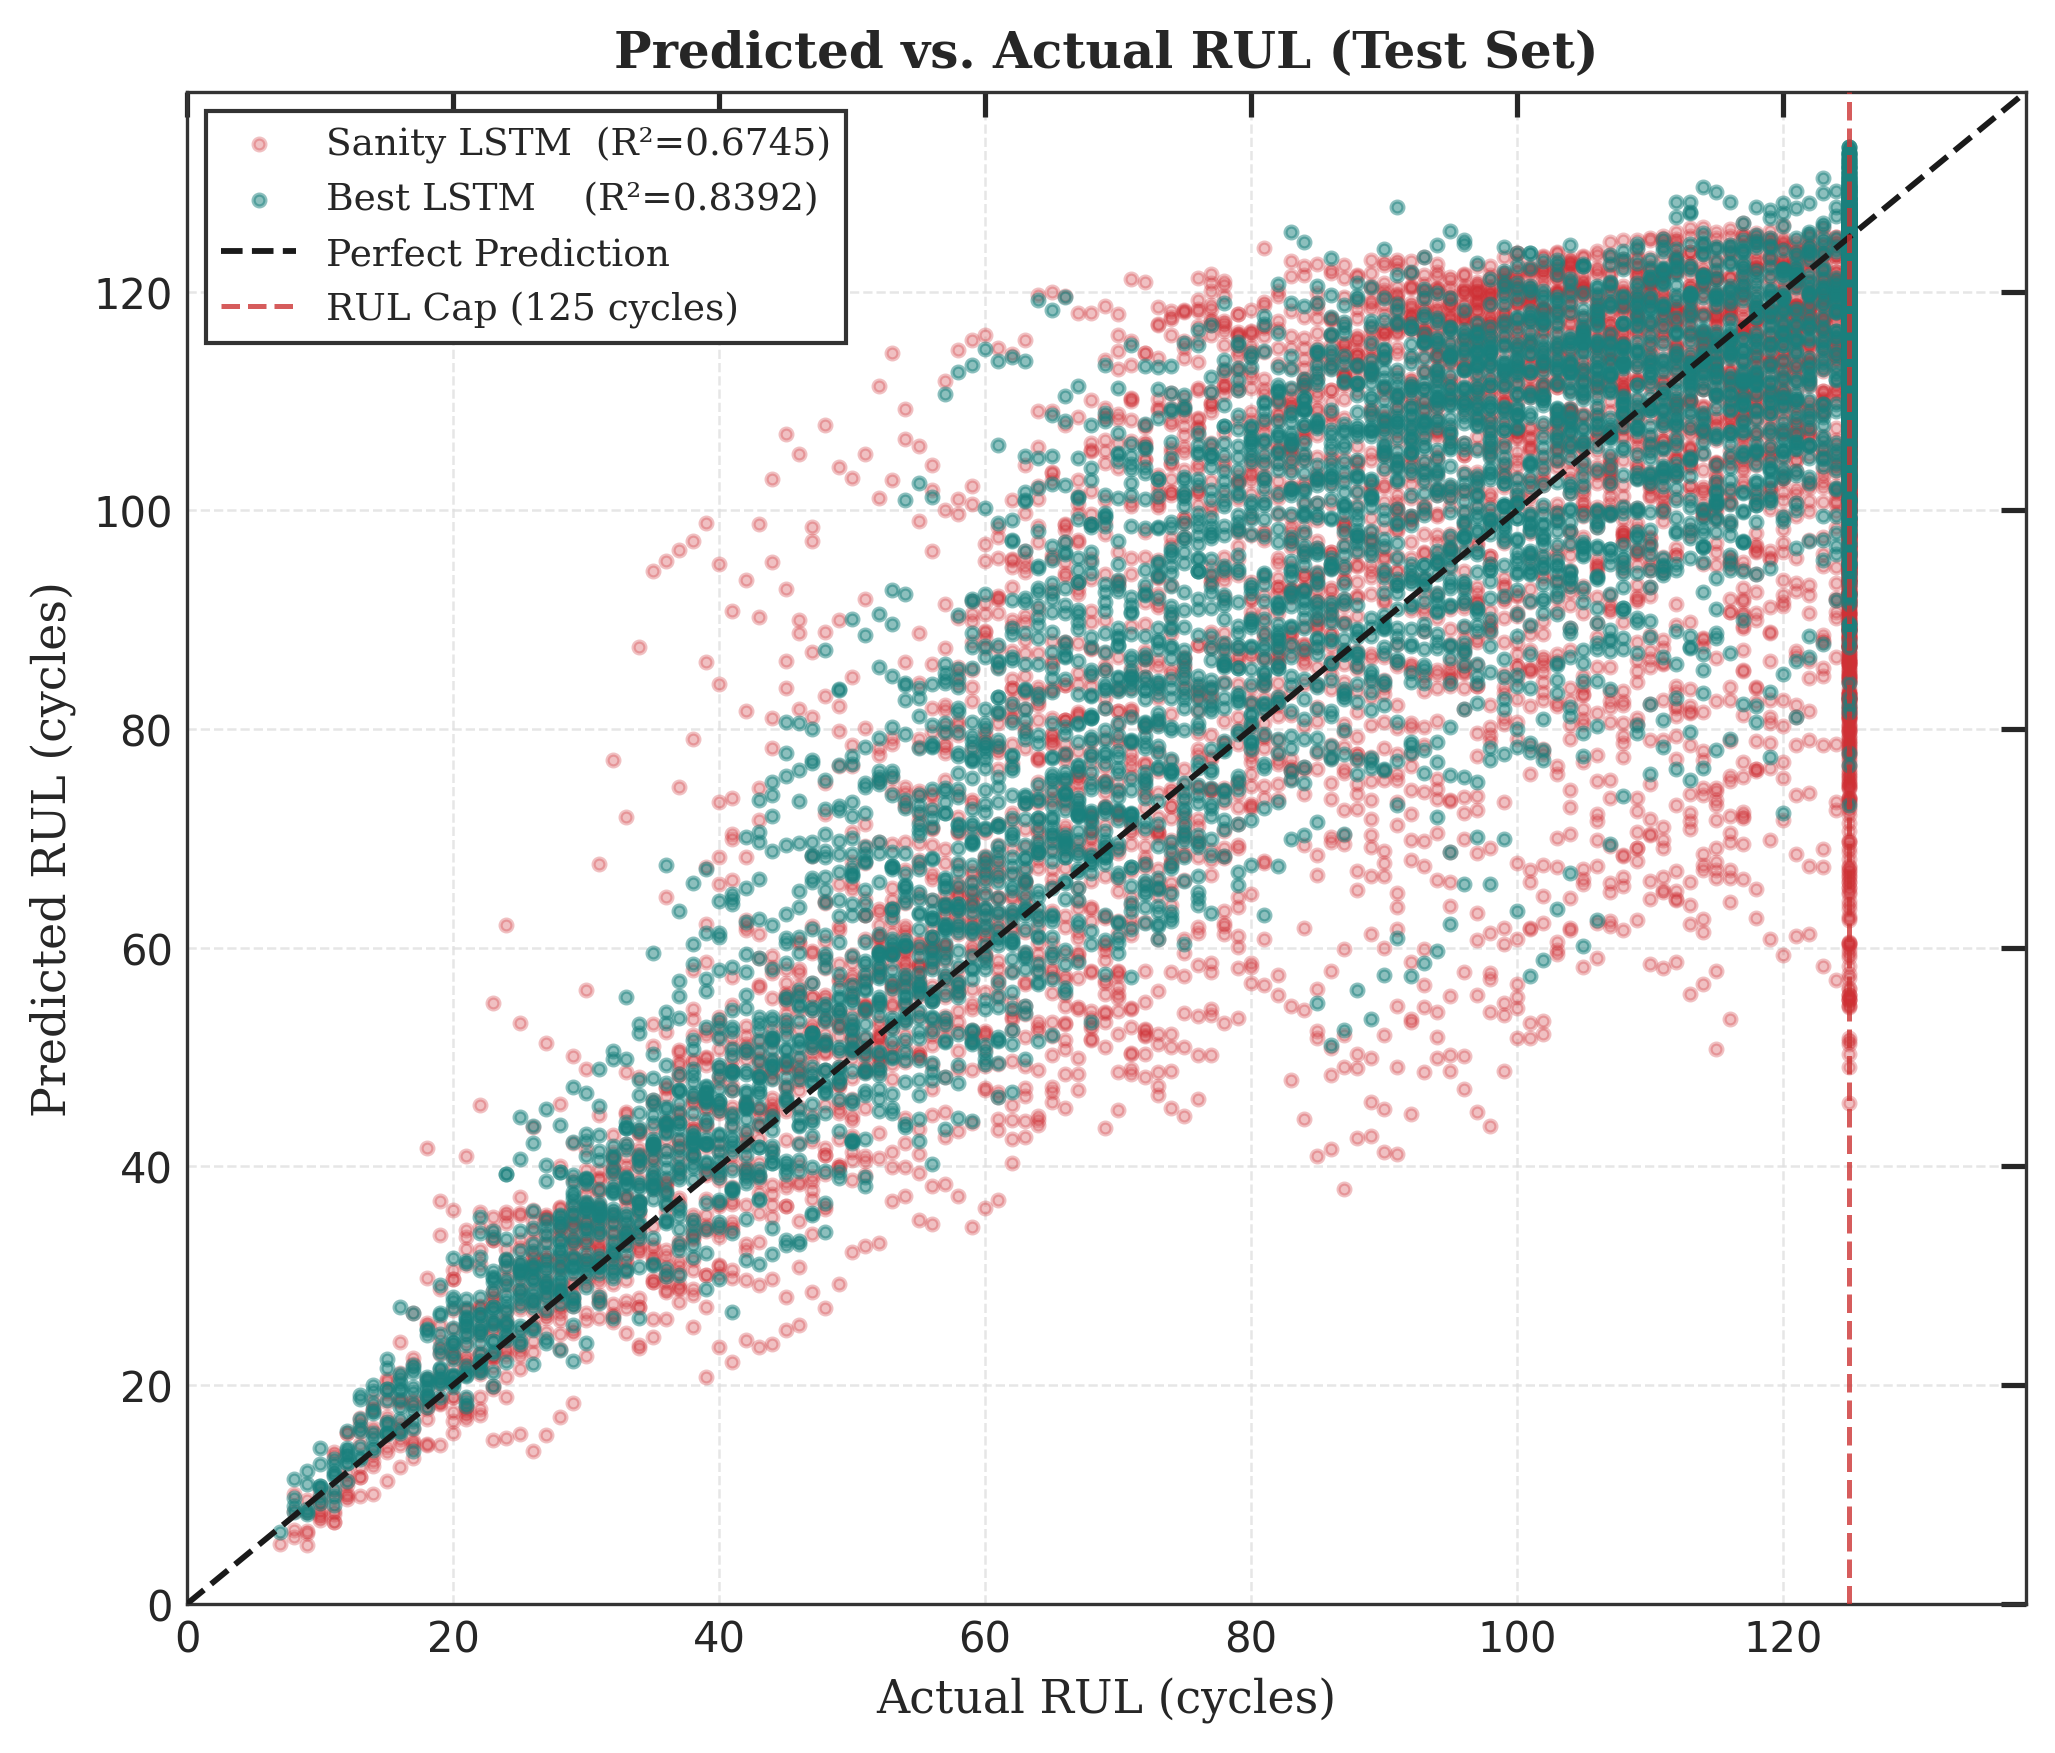
\includegraphics[width=0.95\linewidth]{lstm_comp_graphs/comparison_scatter_sanity_vs_best_lstm.png}
    \caption{Predicted vs. Actual RUL: Sanity vs. Best LSTM (Test Set)}
    \label{fig:comp_scatter}
\end{figure}

The residual distributions (Fig.~\ref{fig:comp_residuals}) confirm this improvement quantitatively. The best LSTM reduces the residual standard deviation from $16.54$ to $13.24$ cycles, with the distribution more tightly centred around zero and substantially reduced tail weight, indicating fewer extreme prediction errors.

\begin{figure}[H]
    \centering
    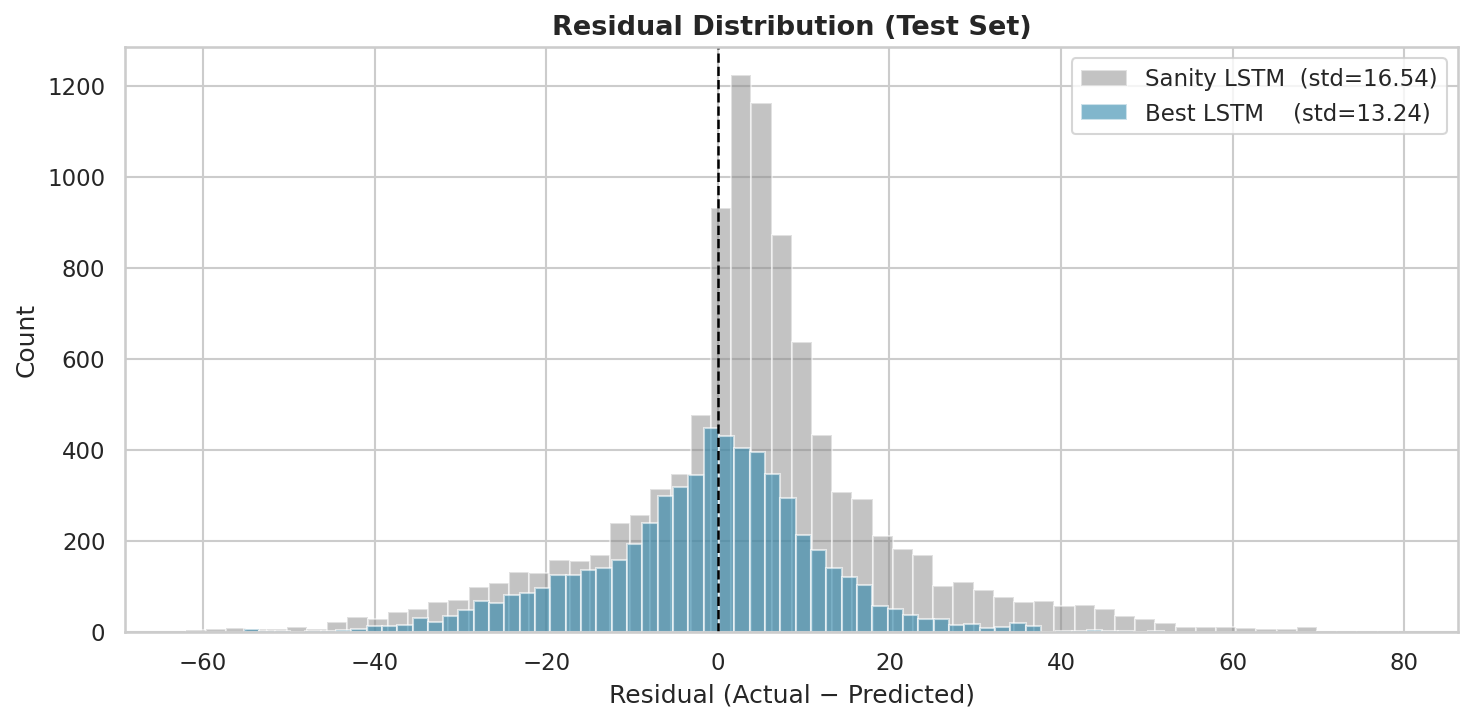
\includegraphics[width=0.95\linewidth]{lstm_comp_graphs/comparison_residuals_sanity_vs_best_lstm.png}
    \caption{Residual Distribution: Sanity vs. Best LSTM (Test Set)}
    \label{fig:comp_residuals}
\end{figure}

The CDF of absolute errors shown in Fig.~\ref{fig:comp_cdf} illustrates that the tuned LSTM achieves $62.4\%$ of test predictions within $10$ cycles, compared to $58.5\%$ for the sanity model. The tuned LSTM CDF curve lies consistently above the sanity curve across all error thresholds, confirming uniform reduction in prediction error magnitude across the full distribution. This improvement is particularly meaningful in a maintenance context, as a greater proportion of predictions falling within a tight error band directly reduces the risk of both premature and delayed maintenance decisions. Taken together, the scatter, residual, and CDF analyses consistently demonstrate that the combination of increased model capacity, extended sequence length, and asymmetric loss training produces a more reliable and practically deployable RUL estimator.

\begin{figure}[H]
    \centering
    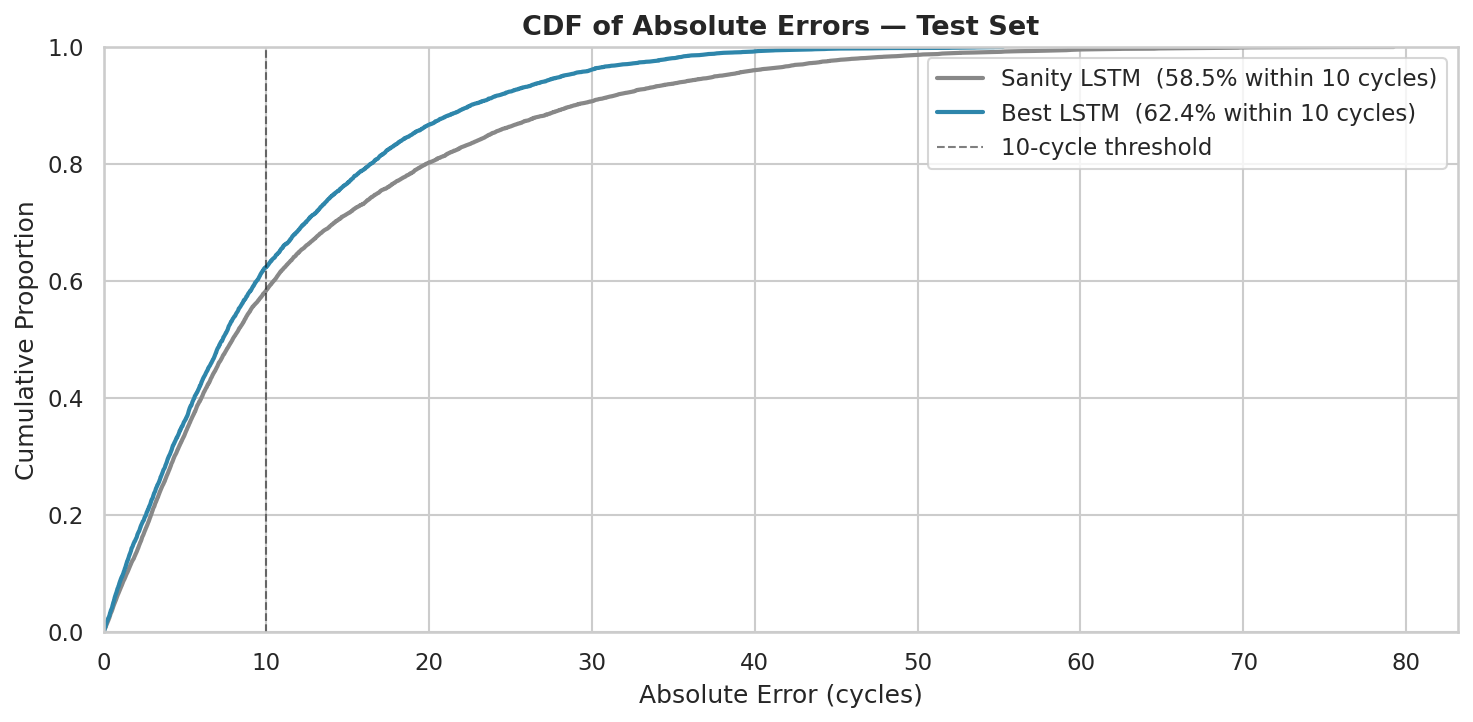
\includegraphics[width=0.95\linewidth]{lstm_comp_graphs/comparison_cdf_sanity_vs_best_lstm.png}
    \caption{CDF of Absolute Errors: Sanity vs. Best LSTM (Test Set)}
    \label{fig:comp_cdf}
\end{figure}

\section{Regularization and Validation}

Achieving strong test performance requires not only a well-tuned architecture but also effective strategies to control overfitting and ensure that validation behaviour transfers reliably to unseen data. This section describes the regularization techniques applied to the tuned LSTM, explains the motivation behind each, and evaluates generalization performance against the broader literature.

\subsection{Regularization Methods}

Three complementary regularization strategies were applied to the final LSTM model to control overfitting and improve generalization:

\textbf{Dropout} \cite{ref8}: A dropout rate of $0.4$ was applied to the LSTM hidden states during training. Each hidden unit is independently deactivated with probability $0.4$ at each training step, preventing co-adaptation of neurons and discouraging reliance on individual recurrent pathways. The higher rate relative to the sanity model ($0.2$) reflects the greater representational capacity of the best LSTM ($296{,}065$ parameters vs.\ $24{,}961$) and the corresponding need for stronger variance regularization.

\textbf{Asymmetric loss} \cite{ref9}: The loss function in Eq.~\eqref{eq:asym_loss} acts as an implicit regularizer by introducing a directional penalty structure. By penalizing overprediction more heavily ($\alpha = 1.5$), it discourages the model from learning overconfident positive biases in high-uncertainty early-degradation regions, where sensor signals are subtle and prediction variance is otherwise largest.

\textbf{Learning rate scheduling}: The \textit{ReduceLROnPlateau} scheduler prevents the optimizer from settling into sharp, poorly generalizing minima by reducing the step size upon stagnation. Halving the learning rate mid-training allowed the model to refine its solution in flatter regions of the loss landscape, which is associated with improved generalization behaviour.

\subsection{Generalization and Comparison with Existing Work}

The validation-to-test R$^2$ drop of $0.0767$ for the final model is substantially lower than that observed for the RF and MLP models (approximately $0.165$ each), indicating that the regularized LSTM generalizes more robustly to unseen engines. The combination of dropout, asymmetric loss, and learning rate scheduling yields a test R$^2$ of $0.8392$ and RMSE of $13.331$ cycles.

These results are competitive with published deep learning approaches to RUL estimation on the FD001 subset. Survey results across LSTM and CNN-based architectures applied to C-MAPSS FD001 report test RMSE values typically ranging from $12$ to $18$ cycles, with the most specialized architectures achieving values near $12$ cycles through attention mechanisms, ensembling, or multi-task loss formulations \cite{ref3}. The final model presented here achieves performance within this range using a single-layer LSTM with standard regularization techniques, demonstrating that disciplined hyperparameter search and asymmetric loss design are sufficient to approach competitive accuracy on FD001 without architectural complexity.

\section{Conclusion}

This paper presented a comprehensive comparison of machine learning and neural network models for Remaining Useful Life (RUL) prediction of turbofan engines. Three models of increasing complexity were developed and evaluated: a Random Forest baseline, a Multilayer Perceptron (MLP), and a Long Short-Term Memory (LSTM) network.

Through systematic evaluation across multiple performance metrics, residual analysis, and hyperparameter sensitivity studies, the following conclusions were drawn:

\begin{itemize}
    \item Baseline models (Random Forest) provide reasonable performance but struggle to capture temporal dependencies, exhibiting compression of predictions at high RUL values.
    \item Neural network approaches (MLP) capture nonlinear patterns more effectively than tree-based methods, achieving modest improvements in validation metrics. However, generalization performance remains limited by the reliance on flattened input representations.
    \item LSTM networks, with proper windowing and normalization, achieve superior RUL prediction accuracy through explicit modeling of temporal degradation patterns, resulting in a substantial reduction in RMSE and improvement in R$^2$ across both validation and test sets.
    \item Significant trade-offs exist between model complexity, computational cost, and predictive performance. While LSTM requires substantially more computational resources during inference, the accuracy improvements justify the additional expense for critical applications such as turbofan engine maintenance.
    \item Hyperparameter optimization via random search, combined with asymmetric loss ($\alpha = 1.5$), learning rate scheduling, and increased dropout ($0.4$), improved the final LSTM to a test R$^2$ of $0.8392$ and RMSE of $13.331$ cycles — a reduction of $3.63$ RMSE cycles over the sanity LSTM and a validation-to-test R$^2$ generalization drop of only $0.077$.
\end{itemize}

The results demonstrate that sequential dependencies in degradation data are a dominant factor in accurate RUL estimation, and that principled regularization is essential for stable generalization to unseen engines. Future work should investigate attention-based mechanisms for further improving temporal representation, ensemble approaches combining multiple models, and domain adaptation techniques for generalization across different C-MAPSS subsets and operating conditions.

\begin{thebibliography}{99}

\bibitem{ref1} A. Saxena and K. Goebel, ``Prognostics and health management of electronics,'' in \emph{Springer Series in Reliability Engineering}, 2017.

\bibitem{ref2} A. Saxena et al., ``Damage propagation modeling for aircraft engine run-to-failure simulation,'' in \emph{Prognostics and Health Management}, 2008.

\bibitem{ref3} W. Zhao, T. Wang, and Y. Ye, ``Deep learning for remaining useful life prediction,'' in \emph{IEEE Reviews in Biomedical Engineering}, vol. 12, pp. 100--115, 2019.

\bibitem{ref4} S. Hochreiter and J. Schmidhuber, ``Long short-term memory,'' \emph{Neural Computation}, vol. 9, no. 8, pp. 1735--1780, 1997.

\bibitem{ref5} C. Teubert, D. Brown, and K. Goebel, ``The ADAPT Toolbox for Real-Time Monitoring and Prediction of Battery RUL,'' in \emph{PHM}, 2016.

\bibitem{ref6} T. Géron, \emph{Hands-On Machine Learning with Scikit-Learn, Keras, and TensorFlow}, O'Reilly Media, 2019.

\bibitem{ref7} I. Goodfellow, Y. Bengio, and A. Courville, \emph{Deep Learning}, MIT Press, 2016.

\bibitem{ref8} N. Srivastava, G. Hinton, A. Krizhevsky, I. Sutskever, and R. Salakhutdinov, ``Dropout: A simple way to prevent neural networks from overfitting,'' \emph{Journal of Machine Learning Research}, vol. 15, pp. 1929--1958, 2014.

\bibitem{ref9} D. Rengasamy, B. Rothwell, and G. P. Figueredo, ``Asymmetric loss functions for deep learning early predictions of remaining useful life in aerospace gas turbine engines,'' in \emph{Proc. Int. Joint Conf. Neural Networks (IJCNN)}, IEEE, 2020, doi: 10.1109/IJCNN48605.2020.9207051.

\end{thebibliography}

\end{document}